\section{Results}

\subsection{Between-Conditions Comparisons}

\subsubsection{Saturation of ideas}

One of our hypotheses (HYP) was that as the number of instances gathered increased, the rate of new ideas, new categories and new singleton categories would converge towards 0.

Figure FIG shows the rate of new idea, category, and non-singleton category generation  over time for each number requested conditions. These plots have been smoothed by randomly shuffling the order in which ideas were receieved 500 times and taking the mean cumulative count at each point in time, and plotting with a window size of 10. In an ideal scenario where each instance provided a new unique idea and category, the lines would horizontal across the top of the figure.

\begin{figure}
    \centering
    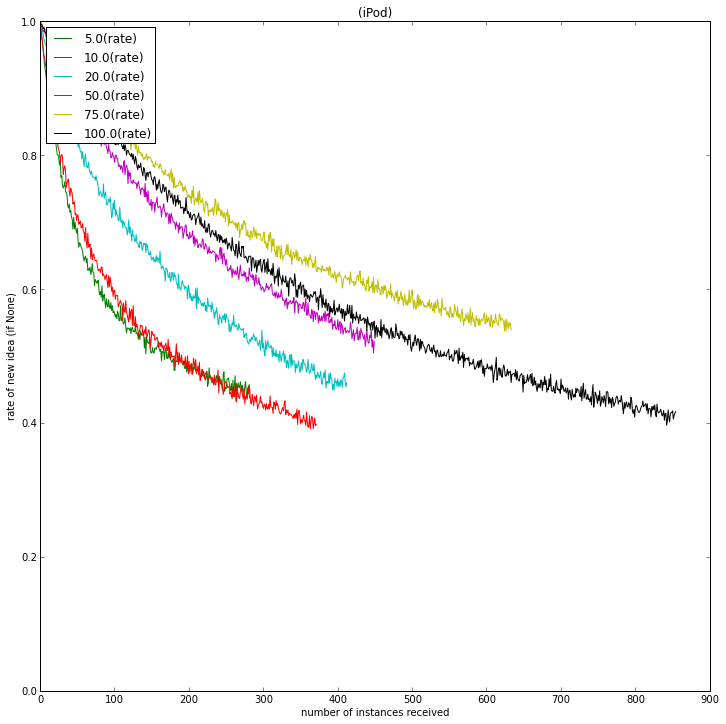
\includegraphics[width=0.9\columnwidth]{rate_new_idea_over_time}
    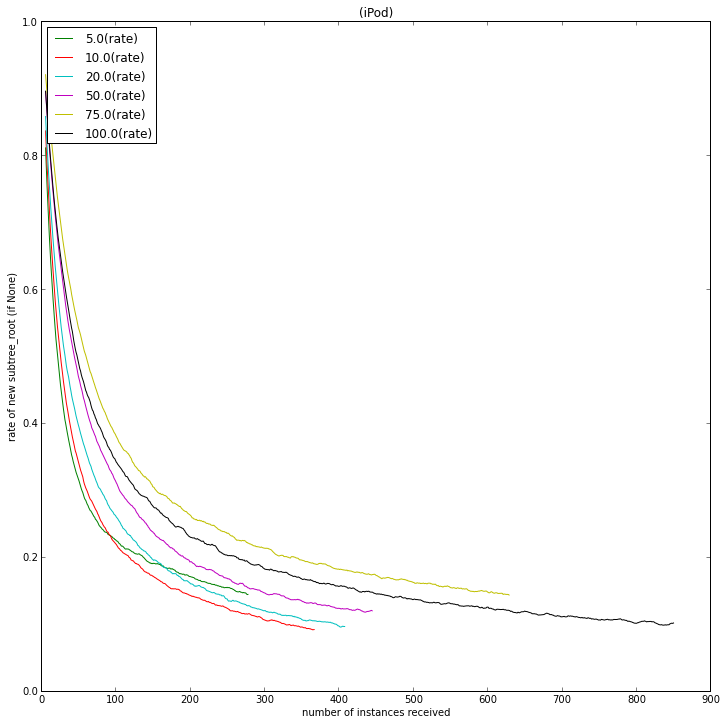
\includegraphics[width=0.9\columnwidth]{rate_new_category_over_time}
    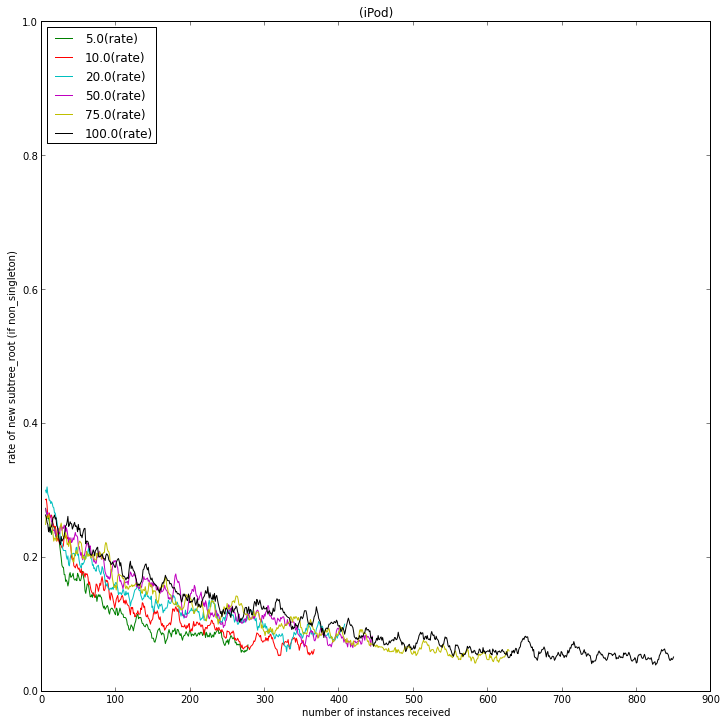
\includegraphics[width=0.9\columnwidth]{rate_new_ns_category_over_time}
    \caption{Rate of idea generation}
\end{figure}

Visually, the rate of idea, category and singleton category generation seems to trend towards 0. We tested this hypothesis...

Additionally Figure FIG indicates that there is some effect of number of ideas requested on the rate of generation. Generally, conditions with more requested responses generated ideas and categories at a higher rate. We tested this...

\subsubsection{Originality}

We were also interested in the effect of the number requested condition on originality. Originality, as measured by o-scores at both the category and idea level, is compared cross condition in figure FIG. Some stat tests here...

\begin{figure}[h]
    \centering
    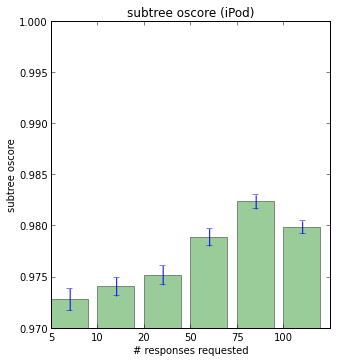
\includegraphics[width=0.9\columnwidth]{subtree_oscore}
    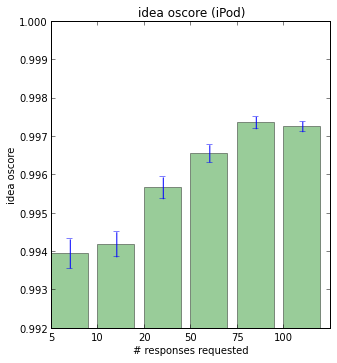
\includegraphics[width=0.9\columnwidth]{idea_oscore}
    \caption{Error bars are standard error}
\end{figure}

The more ideas requested, the more original the ideas produced. This provides support for the findings of Parnes et al \cite{parnes_effects_1961}, namely that more original ideas are found in extended idea generation events. This finding will be examined in the next section.

\subsubsection{Generality}

As discussed above, we use height in category tree as a measure of an ideas generality. Generality (and its reverse, sepcificity) are both potentially desireable outcomes of a brainstorming task.

The idea-height across number conditions is given in figure FIG.

\begin{figure}[h]
    \centering
    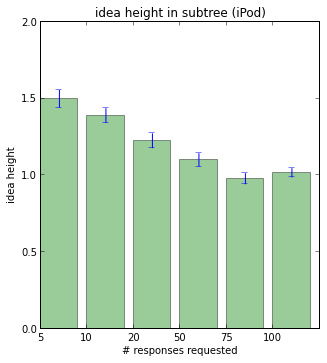
\includegraphics[width=0.9\columnwidth]{height_in_subtree}
    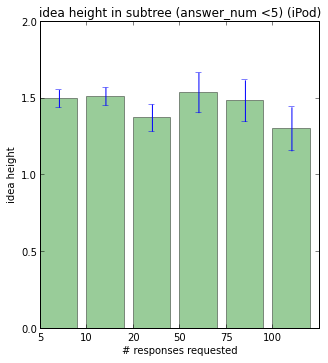
\includegraphics[width=0.9\columnwidth]{height_in_subtree_5}
    \caption{Generality of ideas}
\end{figure}

The top panel in Figure FIG suggests that ideas tend to be less general in the conditions where we request more ideas. However, the bottom panel, which shows generality only for the first 5 responses, has no such effect. This suggests that only answers later on in the larger request batches become less general, an effect that we further examine in the following section.

In this previous section, we showed that the rate of idea convergence, the originality of ideas, and the generality of ideas varied between the number requested conditions. These relationships are useful to understand when deciding what crowd brainstorming strategy to follow. What this birds eye view excludes is an understanding of \emph{how} these differences occur. To that end, we shift our attention to the context of a single brainstorming run.

\subsection{Brainstorming Runs}

The large, experiment-scale trends we describe above are composed of ideas generated in many individual brainstorming runs.

\subsubsection{Originality}

In the previous section, we showed that originality at both the idea and category tree level rose as the number of responses solicited increased. Parnes et al fround that ideas generated in the latter half of a brainstorming session were rated more original in colocated, cotemporal idea generation groups \cite{parnes_effects_1961}. We hypothesize that we should see a difference in idea and category oscore as a function of position in the brainstorming run, with later ideas performing better. Figure FIG presents the mean oscroe ratings on this scale.

\begin{figure}[h]
    \centering
    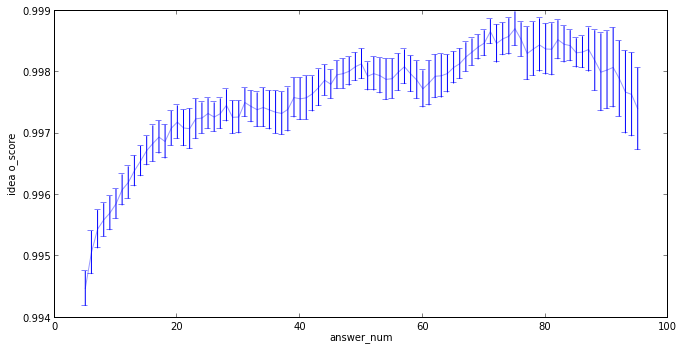
\includegraphics[width=0.9\columnwidth]{run_idea_oscore}
    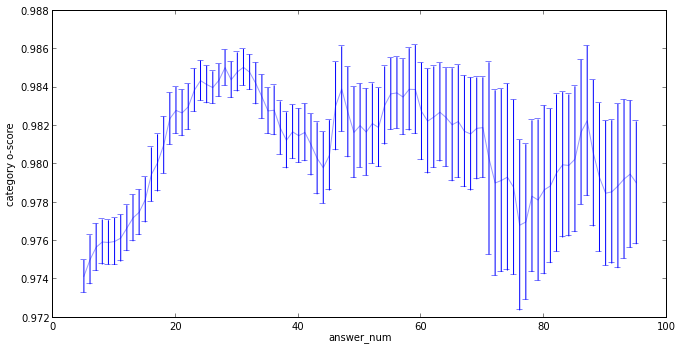
\includegraphics[width=0.9\columnwidth]{run_category_oscore}
    \caption{Error bars are standard error}
\end{figure}

There appears to be a clear, uniform increase in originality on both measures through the 20th idea, at which point originality peters out, or, in the case of category o-score, becomes highly variant. We tested the hypothesis that ideas were less creative after the 20th...

Thus, we confirm Parnes et al's prior result: later ideas are more original than those early in the run. Furthermore, we identify 20 ideas as a key inflection point past which participants have realiably exhausted their supply of readily available ideas and begin generating their most original ideas.

\subsubsection{Generality}

Similarly, generatility was found to decrease as the number of ideas requested increased. Figure FIG shows generality over the course of a brainstorming run.

\begin{figure}[h]
    \centering
    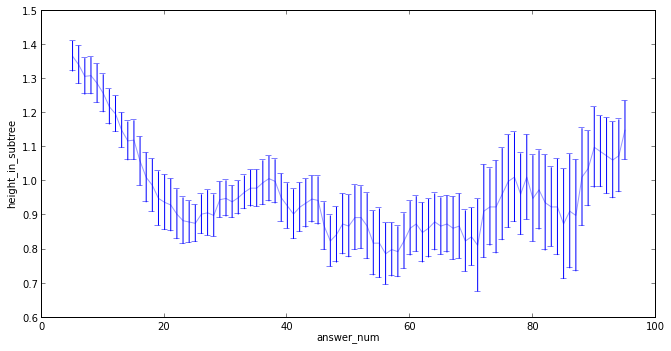
\includegraphics[width=0.9\columnwidth]{run_height_in_subtree}
    \caption{Error bars are standard error}
\end{figure}

Unsurprisingly, generality performs inversely to originality - the most general ideas are the least original. Also like originality, participants seem to exhaust their supply of general ideas by around the 20th idea, at which point they produce ideas at a fairly uniform generality. We tested this...

\subsubsection{SIAM hypotheses}

\cite{nijstad_how_2006}